%% \documentclass[runningheads]{llncs}
\documentclass{bmcart}

% Paquetes de la AMS:
%% \usepackage{amsmath, amsthm, amsfonts, amssymb}
%\usepackage{amsmath}
%\usepackage{amsfonts}
%\usepackage{amssymb}
%% \usepackage{authblk} % para los autores y las afiliaciones
%%% \usepackage{array}
%\usepackage[english]{babel}
%%% \usepackage{fullpage}
%\usepackage{graphicx}
%\usepackage[utf8]{inputenc}
%\usepackage{mathtools}
%%% \usepackage{subcaption} % subfigures
%\usepackage[caption=false]{subfig}
%\usepackage{url}

\usepackage{amsthm,amsmath}
\usepackage{amsfonts}
\usepackage{graphicx}
\usepackage[utf8]{inputenc}

\usepackage{todonotes}
\usepackage{lmodern}  % font sizes
\usepackage{hyperref} % ref unlabeled sections

\def\RR{\mathbb{R}}
\def\ZZ{\mathbb{Z}}
\newcommand{\abs}[1]{\left\vert#1\right\vert}



\begin{document}

\begin{frontmatter}

\begin{fmbox}
\dochead{METHODOLOGY}


%Enter the title of your article here
\title{An Analysis of Overlapping Communities for
  Identifying Stress Responsive Genes}

% Authors
\author[
  addressref={aff1},                        % id's of addresses, e.g. {aff1,aff2}
  corref={aff1},                            % id of corresponding address, if any
% noteref={n1},                             % id's of article notes, if any
  email={camila.riccio@javerianacali.edu.co}   % email address
]{\inits{C.R.}\fnm{Camila} \snm{Riccio}}
\author[
  addressref={aff2},
  email={jfinke@javerianacali.edu.co}
]{\inits{J.F.}\fnm{Jorge} \snm{Finke}}
\author[
  addressref={aff2},
  email={camilo.rocha@javerianacali.edu.co}
%]{\inits{C.R.}\fnm{Camilo} \snm{Rocha}}
]{\inits{H.C.R.}\fnm{Camilo} \snm{Rocha}}

% Authors' addresses
\address[id=aff1]{%                                         % unique id
  \orgdiv{Department of Natural Sciences and Mathematics},  % department, if any
  \orgname{Pontificia Universidad Javeriana},               % university, etc
  \city{Cali},                                              % city
  \cny{Colombia}                                            % country
}

\address[id=aff2]{%                                         % unique id
  \orgdiv{Department of Electronics and Computer Science},  % department, if any
  \orgname{Pontificia Universidad Javeriana},               % university, etc
  \city{Cali},                                              % city
  \cny{Colombia}                                            % country
}


\end{fmbox}% comment this for two column layout

\begin{abstractbox}

\begin{abstract} % abstract
\parttitle{Background} %if any
This paper proposes a workflow to identify which genes respond to
  specific treatments in plants.
  The workflow takes as
  input the RNA sequencing read counts and phenotypical data of different genotypes,
  measured under  control and treatment conditions.
  It outputs a reduced group of genes marked as relevant for
  treatment response. Technically, the proposed approach is both a
  generalization and an extension of 
%  Weighted Gene Co-expression Network Analysis (WGCNA).
  WGCNA.
  It aims to 
  identify specific modules of overlapping communities underlying the co-expression network of genes.
  Module detection is
  achieved by using Hierarchical Link Clustering.
  Identifying such modules enables us to take into account
  the overlapping nature of the regulatory domains of the systems that generate
  co-expression. LASSO regression is employed to analyze
  phenotypic responses of modules to treatment.

\parttitle{Results} %if any
  The workflow is applied to rice
  (\textit{Oryza sativa}), a major food source known to be
  highly sensitive to salt stress.
  The workflow identifies 19 rice genes that seem
  relevant in the response to salt stress.
  They are
  distributed across 6 modules: 
  3 modules, each grouping together 3 genes, are associated to shoot K content;
  2 modules of 3 genes, are associated to shoot biomass;
  and 1 module of 4 genes is associated to root biomass.
  These genes represent target genes for the improvement of
  salinity tolerance in rice.
   
  
\parttitle{Conclusions}
A more effective framework to reduce the
  search-space for target genes that respond to a specific treatment is introduced.
  It facilitates experimental validation by restraining efforts to
  a smaller subset of genes of high potential relevance.
  
\end{abstract}

% keywords
% Put each keyword in separate \kwd{}
\begin{keyword}
\kwd{Stress-responsive genes}
\kwd{co-expression network}
\kwd{overlapping communities}
\kwd{phenotypic traits}
\kwd{LASSO}
\kwd{salinity}
\kwd{rice}
\kwd{\textit{Oryza sativa}}
\end{keyword}

\end{abstractbox}

\end{frontmatter}


\section*{Introduction}
\label{sec.intro}

Stresses are key factors that influence plant
development, often associated to extensive
losses in agricultural production~\cite{mesterhazy2020losses, shrivastava2015soil}. 
Soil salinity is one of the
most devastating abiotic stresses. According to~\cite{shrivastava2015soil}, 
soil salinity contributes to a significant reduction in areas of cultivable
land and crop quality. The study estimates that 
20\% of the total cultivated land worldwide and 
33\% of the total irrigated agricultural land
is affected by high salinity. 
By the end of 2050 areas of high salinity are
expected to reach 50\% of the cultivated land~\cite{shrivastava2015soil}. 
\vspace{0.5cm}

Salinity tolerance and
susceptibility are the result of elaborated
interactions between morphological, physiological, and biochemical
processes, which are regulated by multiple genes in
various parts of the plant genome~\cite{reddy2017salt}. Consequently,
identifying groups of responsive genes is an important step in efforts to
improve crop varieties in terms of salinity tolerance.
This paper proposes a workflow to identify stress responsive genes
associated with a complex quantitative trait.
\vspace{0.5cm}

To discover which genes are associated with a phenotypic response to
treatment the workflow takes as input
the gene expression profiles of the target organism, specifically, 
the RNA sequencing read counts (measured under control
and treatment conditions)
of at least two biological replicates per genotype. It also receives phenotypic data, specifically, observable traits, measured for each genotype under the two conditions. The output of the
workflow is a set of genes which are characterized as potentially relevant
to treatment. 
\vspace{0.5cm}

Broadly speaking, the workflow provides a framework that yields insight into the possible behavior of specific
genes and the role they play in functional pathways in response to
treatment. 
It takes advantage of
the current availability of high-throughput technologies, which
enables the access to transcriptomic data of organisms under different conditions, 
and a better understanding of their reaction under different
environmental stimuli.
\vspace{0.5cm}

The proposed approach is both a generalization and an
extension of the widely applied workflow 
for identifying target genes called 
Weighted Gene Co-expression Network Analysis
(WGCNA)~\cite{langfelder2008wgcna, tian2018identifying}.
Like WGCNA, the general idea behind the proposed
approach is to identify, after a sequence of normalization
and filtering steps, specific modules of overlapping communities
underlying the co-expression network of genes. 
The proposed approach is considered a \textit{generalization}
of WGCNA because module detection recognizes overlapping communities
using Hierarchical Link Clustering (HLC)~\cite{ahn2010link} algorithm.
Conceptually, the generalization takes into account
the overlapping nature of the regulatory domains of the
systems that generate the co-expression network~\cite{gaiteri2014beyond}.
More specifically, overlapping modules allow for 
scenarios where biological components  are involved in
multiple functions.
\vspace{0.5cm}

The workflow is also an \textit{extension} of WGCNA
because two additional constraints are considered:
networks in the intermediate steps are forced to be
scale-free~\cite{barabasi2003scale}, and LASSO
regression~\cite{tibshirani1996regression} selects the
most relevant modules of responsive genes.
The regularized regression technique of LASSO
forces the less relevant variables to be associated to regression
coefficients of value zero~\cite{desboulets2018review}, 
which is of interest
in scenarios where the number of variables is much larger than
the number of samples. This condition is satisfied when the target variables represent the
overlapping communities (obtained with HLC) and the samples represent genotype data,
which is usually a small set due to the high cost of the RNA sequencing process. 
Finally, the proposed workflow is also modular, since other module detection
and selection techniques could be explored instead HLC and LASSO.
\vspace{0.5cm}

The approach is showcased with a systematic study on rice
(\textit{Oryza sativa}), a food source that is known to be
highly sensitive to salt stress~\cite{chang2019morphological}. RNA-seq
data was accessed from the GEO database~\cite{clough2016gene}
(accession number GSE98455). It represents $57845$ gene expression
profiles of shoot tissues measured under control and stress conditions
in $92$ accessions of the Rice Diversity Panel 1~\cite{eizenga2014registration}. A total of 6 modules
are detected as relevant in the response to salt stress in rice: 3
modules, each grouping together 3 genes, are associated to shoot K content; 2
modules of 3 genes, are associated to shoot biomass; and 1 module of 4
genes is associated to root biomass. These genes are potential
targets for experimental validation of salinity tolerance. 
From the 19 genes, 16
are also identified as deferentially expressed for at least
one of the 92 accessions, which re-enforces the labelling of the genes as
stress responsive. Only 2 of the 16 differentially
expressed genes, associated to shoot biomass, are
named and known to produce protein products: spermidine
hydroxycinnamoyltransferase~2 (SHT2) and lipoxygenase. 
Further studies are needed to elucidate the detailed biological
functions of the remaining 14 genes and their role
in the mechanisms that respond 
to salt conditions.

\paragraph{Paper Outline.}
%The remainder of the paper is organized as
%follows. Section~\ref{sec.prelim} gathers preliminaries on gene
%co-expression networks, HLC, and LASSO. The proposed workflow is
%presented in Section~\ref{sec.framework}, with especial focus on the
%logical steps of the process and the internal structures supporting
%the approach. Section~\ref{sec.case} presents the case study on the
%identification of rice genes that are sensitive to salt
%stress. Section~\ref{sec.concl} draws some conclusions and future research directions.

The remainder of the paper is organized as
follows. The \hyperref[sec.prelim]{Preliminaries} section gathers foundations on gene
co-expression networks, HLC, and LASSO. The proposed workflow is
presented in \hyperref[sec.framework]{the Workflow} section, which enphasizes on the
logical steps of the data analysis process and the internal structures supporting
the approach. The \hyperref[sec.case]{Case Study} section presents an application of the workflow for the
identification of rice genes that are sensitive to salt
stress. Finally, the \hyperref[sec.concl]{Concluding Remarks} section draws some conclusions and future research directions.

\section{Preliminaries}
\label{sec.prelim}

This section presents preliminaries on networks, hierarchical link
clustering and the LASSO linear regression technique.

\subsection{Co-expression network}

A network is an undirected graph $G=(V,E)$ where
${V=\{v_1,v_2,\ldots,v_{n}\}}$ is a set of \textit{vertices} or
\textit{nodes} and ${E=\{e_1,e_2,\ldots,e_q\}}$ is a set of
\textit{edges} or \textit{links} that connect vertices. In a gene
co-expression network, each node corresponds to a gene. A pair of
genes is connected if they show similar expression
patterns. A simple and unweighted network can be represented by an
adjacency matrix $A \in \{0,1\}^{n \times n}$ that is symmetric with a
positive one in the positions $(v_i,v_j)$ and $(v_j,v_i)$ whenever
there is an edge connecting vertices $v_i$ and $v_j$, and zeros
elsewhere. Co-expression networks are of biological interest because
the co-expressed genes are usually controlled by the same
transcriptional regulatory pathway, functionally related or members of
the same pathway or metabolic complex.


\subsection{Hierarchical Link Clustering}

The Hierarchical Link Clustering (HLC) algorithm was proposed by Ahn
et al.~\cite{ahn2010link}. The HLC approach represents communities as
groups of links (rather than nodes), and each node inherits all
memberships of its links and can thus belong to multiple, overlapping
communities. It maps links to nodes and connects them if a pair of
links shares a node. The similarity between two links $e_{ik}$ and
$e_{jk}$ is computed using the Jaccard index
%
\begin{equation}\label{eq:jaccard}
  S(e_{ik},e_{jk}) = \frac{\vert n(i) \cap n(j) \vert}{\vert n(i) \cup n(j) \vert},
\end{equation}
%
where $n(i)$ denotes the set containing exactly node $i$ and its
neighbors. The algorithm uses single-linkage hierarchical clustering
to build a dendrogram in which each leaf is a link from the original
network and branches represent link communities. Hierarchical
clustering algorithms repeatedly merge groups until all elements are
members of a single cluster. For the purpose of finding meaningful
communities, it is crucial to know where to partition the
dendrogram. In this case, the most relevant communities are
established at the maximal partition density $D$, a function based on
link density inside communities measuring the quality of a link
partition. The partition density $D$ has a single global maximum along
the dendrogram in almost all cases, because its value is the average
density at the top of the dendrogram (a single giant community with
every link and node) and it is very small at the bottom of the
dendrogram (most communities consists of a single link). In
particular, it is the case that $D = 1$ when every community is a
fully connected clique and $D = 0$ when each community is a tree. If a
community is less dense than a tree (i.e. when the community subgraph
has disconnected components), then such a community contribute
negatively to $D$, which can take negative values. The minimum density
inside a community is $-2/3$, given by one community of two
disconnected edges. Since $D$ is the average of the intra-community
density, there is a lower bound of $-2/3$ for $D$. Computing $D$ at
each level of the link dendrogram can help the purpose of picking the
best level to cut, although meaningful structure could exist above or
below the threshold. The output of cutting is a set of node clusters,
where each node can participate in multiple communities.

\subsection{Least Absolute Shrinkage Selector Operator}

The Least Absolute Shrinkage Selector Operator (LASSO) is a
regularized linear regression technique. It combines a regression
model with a procedure of contraction of some parameters towards zero
and selection of variables, imposing a restriction or a penalty on the
regression coefficients. In other words, LASSO solves the least
squares problem with restriction on the $ L_1$-norm of the coefficient
vector. It can be especially useful to solve problems where the number
of variables (e.g., genes) $ n $ is much greater than the number of
samples $ m $ (i.e., $ n \gg m $).

Consider a dataset consisting of $m$ samples, each of which consists
of $n$ covariates and a single outcome. Let $y_i$ be the outcome and
$x_i := (x_1,...,x_n)$ be the covariate vector for the $i$-th
sample. The objective of LASSO is to solve
%
\begin{equation}
\min \left\lbrace\sum_{i=1}^{m}{\left( y_i-\sum_{j=1}^n{\beta_j
    x_{ij}}\right)^2} \right\rbrace \quad , \quad \textrm{subject to}
\quad \sum_{j=1}^n\abs{\beta_j}\leq s.
\end{equation}

Equivalently, in the Lagrangian form, it minimizes

\begin{equation}
  \sum_{i=1}^{p}{\left( y_i-\sum_{j=1}^n{\beta_j x_{ij}}\right)^2} +
  \lambda \sum_{j=1}^n\abs{\beta_j}
\end{equation}
%
where $s$ is the regularization penalty and $\lambda \geq 0$ is the
corresponding Lagrange multiplier. Since the $\lambda$ value
determines the degree of penalty, the accuracy of the model depends on
its choice. Cross-validation is often used to select the
regularization parameter, choosing the one that minimizes the
mean-squared error.


% Model framework - similar to materials and methods, but with more paragraph
% continuity

\subsection*{Framework Conception and Configuration}

As mentioned before, the functionality of a protein strongly depends on its 3D structure, 
so that changes in its conformation (mutations) can affect how a protein interacts with its 
surroundings \cite{Sikosek2014Prot}. In this aspect, $A_G$ gives intrinsic information 
about complementarity between pairs of proteins and hence paths on the protein network are 
relevant for the prediction task. 

The proposed framework for prediction of protein-protein interactions consists of the
combination of the path counting metrics along with the vector representations of the
edges of the network (node2vec embeddings). Namely, the path counting metrics are either 
the counting of paths of length 2 (matrix $A_G^2$), the counting of paths of length 3 
(matrix $A_G^3$) or the degree-normalized counting of paths of length 3 (matrix $L_3$). 
The information retrieved from these matrices will be addressed from now on as A2, A3 
and L3, respectively.

Figure \ref{fig:framework} shows the proposed framework for predicting protein-protein interactions. As the 
framework combines two sources of information, it consists of three processes: (a) Metrics 
calculation and initial predictions, (b) Node and edge embeddings and (c) Machine Learning 
prediction.

\begin{figure}[h]
\caption{\label{fig:framework}Framework scheme}
	\includegraphics[width=\textwidth ]{figures/framework.eps}
\end{figure}

The input for the workflow consists of a representation of the connectivity of the network.
Online databases of protein-protein interactions usually report this information as an 
adjacency list with some additional attributes about the quality of this interaction. Namely, 
this data is represented as a list of pairs of identifiers and zero or more attributes for 
each pair. The framework only needs to know whether an interaction exists and therefore this 
additional information needs to be discarded in advance. In order to calculate optimally the
subsequent metrics, the framework creates the adjacency matrix $A_G$ out of the given list. 
Note that as no attributes from nodes or edges are added, the framework predicts based only 
on the intrinsic properties of the network related to connectivity. 

\subsubsection*{A. Metrics Calculation}
The goal of this stage is to build matrices $A2$, $A3$ and $L3$ which quantify, 
the number of paths of length 2, of length 3 and the degree-normalized count of 
paths of length 3, respectively. For this purpose, two calculations are done: 
counting the degree of each node ($k_i \in \mathbb{Z}$) and raising $A_G$ to the 
second to obtain $A2$. Finally, $A3$ and $L3$  are calculated simultaneously. 
Entries $L3_{i,j}$ of $L3$ can be calculated as 

\begin{equation}
  L3_{i,j}=\sum_{p,q\in V}\frac{{A_G}_{i,p}\cdot {A_G}_{p,q}\cdot {A_G}_{q,j}}{\sqrt{k_{p}\cdot k_{q}}}
\end{equation}

\subsubsection*{B. node2vec Embeddings}
The purpose of this step is to retrieve a vector representation of the network 
structure and thus be able to feed the Machine Learning model and improve its 
predictions. This is done using a state-of-the-art algorithm called node2vec, 
which is based on the word2vec technique to learn learn word associations from
a corpus of text. Instead of sentences, node2vec uses 
random walks from each node in order to construct a skip-gram model and a neural 
network to learn features (embeddings) from the nodes\cite{Grover_2016}. These 
features consist of a $d$-dimensional vector representation of each node.
Since the framework aims to predict edges, these node embeddings are used as 
input for the Hadamard operator to calculate edge embeddings. Namely, the edge 
embedding of edge $c_i,j$ is calculated as the element-wise product of each 
component of the node embeddings for nodes $i$ and $j$. $d$ is chosen as 16.

\subsubsection*{C. Machine Learning Prediction}
Finally, this stage aims at gathering information from the previous steps to 
enrich the prediction of a Machine Learning (ML) model and improve its results. 

The selected implementation for this prediction problem is XGBoost, which 
uses gradient boosted decision trees to learn whether an interaction is feasible. 
The first step in this process is to combine the two sources of information into 
Dataframes for each of the metrics: for each edge, the information from one of the 
metrics (A2, A3 or L3) is appended to the vector representation of $d$ dimensions 
from node2vec, resulting in 3 different tables. Dataframes including only one 
source of information (each metric or node2vec data) are also generated and 
fed to XGBoost for comparison.

For each metric, the initial prediction in step A is used to train the supervised 
ML model 


\subsection*{Framework Evaluation on the Human Interactome}

As the first step in the evaluation of A2, A3 and L3 metrics to assess link
prediction, the full calculation and ranking of all predictions was
carried out. The results for the analyzed human interactomes (\emph{HI-II-14}
and \emph{HI-TESTED}) is shown in Figure \ref{fig:HI1}, in which
the x axis represents a rank position $k$ and the y axis displays
the precision for the top $k$ predictions of each method, when assuming
interactome \emph{HI-III} as the validation set. 
	
\begin{figure}[h]
\caption{\label{fig:HI1}Methods Comparison for \emph{HI-II-14} and \emph{HI-TESTED}}
	\includegraphics[width=\textwidth ]{figures/figure2.eps}
	%\includegraphics[width=0.7\textwidth ]{../hi-tested.txt.}
\end{figure}

As it can be inferred from the plots, L3-based predictions outperform
their $A{{}^2}$ counterparts. Results also show that L3-score and
$A^{3}$predictions follow a very similar trend.

However, the interest of this study is to assess if Machine Learning can boost
the overall performance on the prediction, so the proposed procedure
is adapted to the human interactome data: Instead of having to remove
a fraction of edges from the network in order to predict and validate,
the prediction network and the validation networks are given beforehand.
The rest of the procedure is carried out as mentioned above.
Table \ref{T1} presents the results for the combinations of Node2Vec
with each feature.

\begin{table}
\caption{\label{T1}Summary statistics for human interactomes}
\includegraphics[width=1\columnwidth]{figures/T1}
\end{table}

In general, performance of all models is above 0.96 in terms of F1-Score.
Although marginally, the A2 feature-enriched model for HI-TESTED performs
better than their counterparts based on paths of length 3. The opposite
is also true for HI-II-14: models enriched with L3 and A3 features
perform better than their A2 counterpart. Results for the Interactome
\emph{HI-II-14} with Node2Vec and each metric are presented in Figures
S\ref{HI1}, S\ref{HI2} and S\ref{HI3}. It can be seen that for
\emph{HI-II-14}, A2 performs marginally better than L3 when comparing
precision but worse in terms of recall, although all metrics have
AUC values of 0.99.

On the other hand, the interactome \emph{HI-TESTED} was assessed with
the same methodology as \emph{HI-II-14} and results are shown in Figures
S\ref{HI1-1}, S\ref{HI2-1} and S\ref{HI3-1}. For this interactome,
A2 performs better in terms of false positives than A3 and L3, but
in terms of false negatives, A3 actually performs better that A2 and
L3. In terms of AUC, metrics results are indistinguishable. 

An interesting assessment from this human datasets can be observed
when looking at the importance plots, which show a very biased influence
of the handcrafted features. Figure \ref{F8-importance-H1} shows
this behavior for the \emph{HI-II-14} dataset, which is very similar
to \emph{HI-TESTED} (Figure S\ref{F8-importance-H2}).

\begin{figure}[h]
\noindent \begin{centering}
\caption{\label{F8-importance-H1}Importance gain plots for \emph{HI-II-14}}
\par\end{centering}
\begin{centering}
\includegraphics[width=0.48\columnwidth]{figures/Human/Imp\lyxdot A2\lyxdot 1\lyxdot eps}\includegraphics[width=0.48\columnwidth]{figures/Human/Imp\lyxdot A3\lyxdot 1\lyxdot eps}
\par\end{centering}
\centering{}\includegraphics[width=0.48\columnwidth]{figures/Human/Imp\lyxdot L3\lyxdot 1}
\end{figure}

% case.tex

For the rice interactome, different combinations of features were
trained on the model and validated. The results are shown in Table
\ref{T2}. First, prediction based on \texttt{Node2Vec} without any
additional feature included is used as baseline of comparison. Figure
\ref{F1} shows those results, and one can see that its mean performance
using the AUC is $0.93$. The results for all 10 repetitions of each
model are consistent, meaning the variance among each line is not
significant. The results for each model using only the default features
are satisfactory. This result can also be assessed when looking at
the confusion matrix, where a precision of $0.98$ and a recall of
$0.86$ are obtained.

\begin{table}
\caption{\label{T2}Summary statistics for rice interactome}
\includegraphics[width=1\columnwidth]{figures/T2.eps}
\end{table}

\begin{figure}[h]
\noindent \begin{centering}
\caption{\label{F1}Summary ROC curves for \texttt{Node2Vec} model alone}
\par\end{centering}
\noindent \raggedleft{}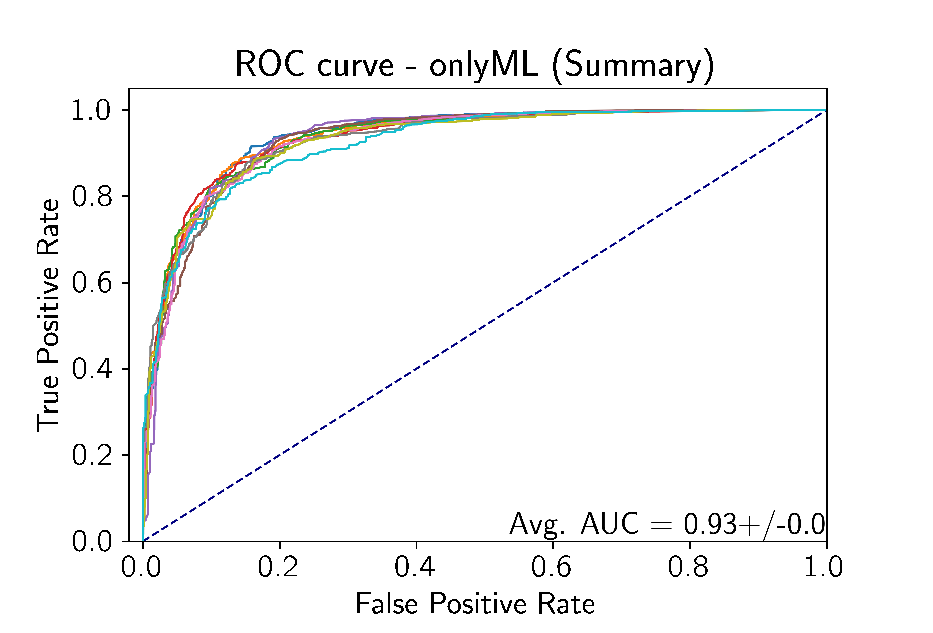
\includegraphics[width=0.48\columnwidth]{figures/Only_ML/ROConlyML_SUMMARY.eps}\includegraphics[width=0.48\columnwidth]{figures/Only_ML/CMonlyML_SUMMARY.eps}
\end{figure}

The next experiment carried out was to add for each prediction method
score as a prediction feature, that is, use the score as an additional
feature for the ML algorithm. Results for the Common Neighbors method
(\textbf{A2}), which uses paths of length 2, are shown in Figure S\ref{F2}.
All 10 experiments have small variability among them and perform better
than the baseline, with AUC of $0.98$. When looking at the confusion
matrix for this model, most guesses are true positives and true negatives,
resulting in a precision of $0.99$ and a recall of $0.91$. The same
analyses are done with the count of paths of length 3 (\textbf{A3})
and with the degree-normalized length-3 score (\textbf{L3}). These
results are presented in figures S\ref{F3} and \ref{F4}, respectively.
The corresponding AUC are $0.97$ and $0.98$.

\begin{figure}[h]
\noindent \begin{centering}
\caption{\label{F4}Results for \texttt{Node2Vec} with L3 feature}
\par\end{centering}
\noindent \raggedleft{}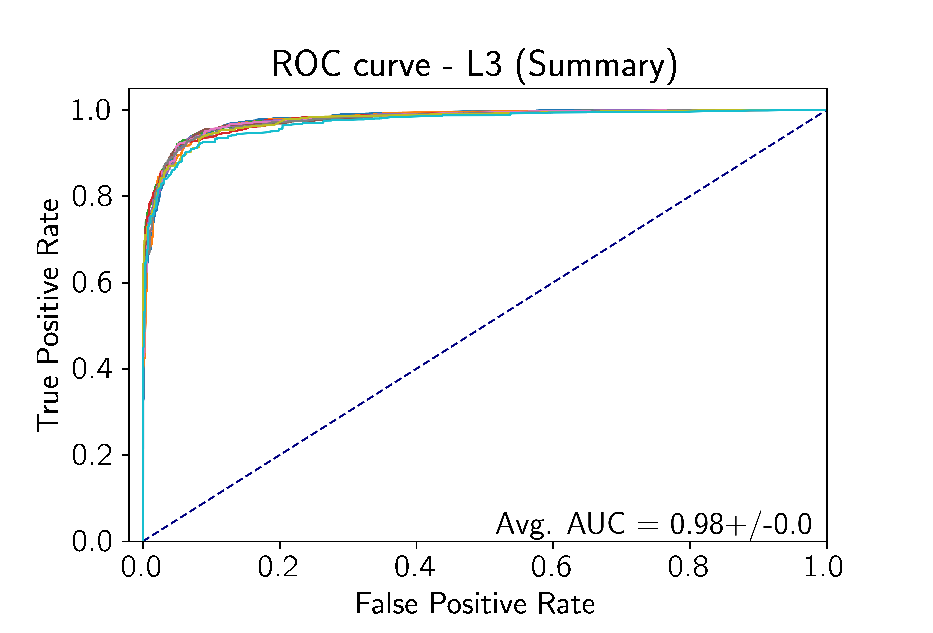
\includegraphics[width=0.48\columnwidth]{figures/ML_Metric/ROCL3_SUMMARY.eps}\includegraphics[width=0.48\columnwidth]{figures/ML_Metric/CML3_SUMMARY.eps}
\end{figure}

The precision when using the count of paths of length 3 (A3) is $0.99$
while the recall is $0.90$. It is interesting to observe that precision
decreased $0.16\%$ and recall decreased $0.58\%$. A similar situation
is obtained for the model with the normalized score (L3), whose precision
decreased to $0.99$ ($-0.08\%$) and recall decreased to $0.88$
($-2.38\%$). It can be seen also that the ROC curve achieves high
values of true positive rate sooner in the A2-featured model than
on the other models.

Another relevant assessment was carried out to verify the predictive
power of the metrics. \texttt{XGBoost} models were trained only using
each metric, for the same 10 experiments. Results are shown in Figures
S\ref{F5}, S\ref{F6} and \ref{F7}. XGBoost yields lower AUC values
when only considering A2, A3 and L3. Precision and recall for this
assessments, although lower than the previous experiments, are still
considered satisfactory.

\begin{figure}[h]
\noindent \begin{centering}
\caption{\label{F7}Results for L3 feature alone}
\par\end{centering}
\noindent \raggedleft{}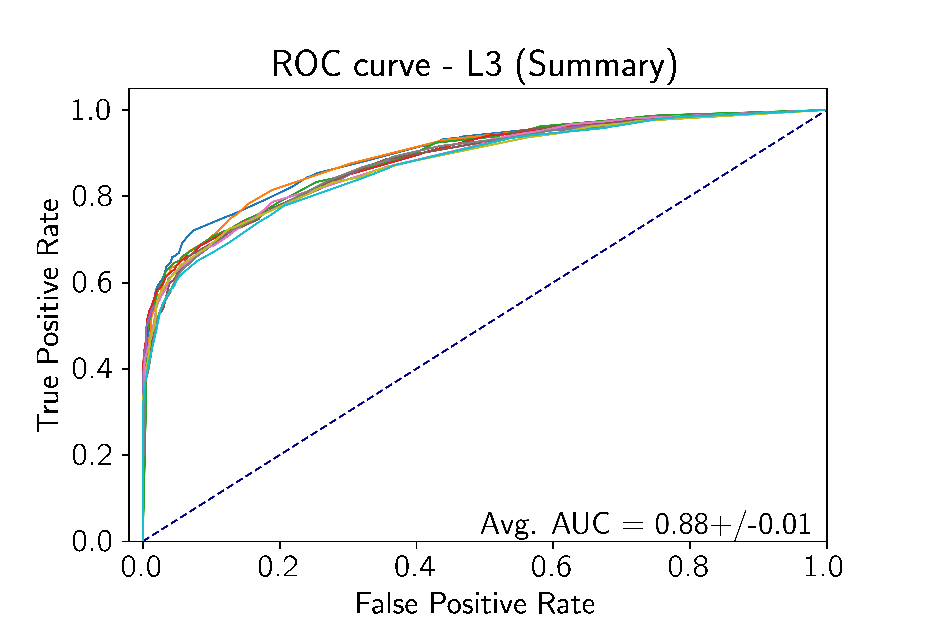
\includegraphics[width=0.48\columnwidth]{figures/Only_Metric/ROConlyL3_SUMMARY.eps}\includegraphics[width=0.48\columnwidth]{figures/Only_Metric/CMonlyL3_SUMMARY.eps}
\end{figure}

Finally, an relevant evaluation on the models that include a handcrafted
feature is necessary: How important is the appended feature for the
model result? The answer can be observed by the feature importance
plots for A2, A3 and L3 in Figure \ref{F8-importance}. Each plot
resembles the importance gain from each feature in the underlying
decision trees that \texttt{XGBoost} uses. Usually, the more bifurcations,
the higher gain a feature has, the more relevance a feature has on
the model prediction itself. All models have the appended feature
as the most important by a good margin, although margin for A3 is
not wide as for A2 or L3.

\begin{figure}[h]
\noindent \begin{centering}
\caption{\label{F8-importance}Importance gain plots for \texttt{Node2Vec}
with each feature}
\par\end{centering}
\begin{centering}
\includegraphics[width=0.48\columnwidth]{figures/ML_Metric/Imp\lyxdot A2\lyxdot All.eps}\includegraphics[width=0.48\columnwidth]{figures/ML_Metric/Imp\lyxdot A3\lyxdot All.eps}
\par\end{centering}
\centering{}\includegraphics[width=0.48\columnwidth]{figures/ML_Metric/Imp\lyxdot L3\lyxdot All.eps}
\end{figure}

\section*{Concluding Remarks}
\label{sec.concl}

This manuscript provides a detailed description of a network-based
analysis workflow for the discovery of key genes responding to a
specific treatment in an organism. It links transcriptomic with
phenotypic data and identifies overlapping gene modules.
\vspace{0.5cm}

The proposed approach is inspired by the workflow suggested in the
WGCNA~\cite{langfelder2008wgcna}. Its main steps are the preprocessing
of the gene expression data, the construction of a co-expression
network, the detection of modules within the network, the relation of
modules with external information (e.g., phenotypic data), and the
enrichment of the identified key genes with additional information.
Both approaches are structured in a modular way, which allows
modifying and exploring different techniques in each step of the
workflow.
\vspace{0.5cm}

The proposed workflow is designed to integrate expression data
measured under two different conditions (namely, control and
treatment), unlike the usually co-expression-based approaches which
work with both conditions independently or consider only a single
condition. For this purpose, an approach similar to that proposed
in~\cite{du2019network} is used, where the control and treatment data
are compiled in a single matrix using the Log Fold Change
measure. Thus, the input to construct the co-expression network is not
the expression data, but instead the changes in the expression levels
from one condition to the other, making room for capturing the signal
of changes caused by the treatment.
\vspace{0.5cm}

An important feature in the proposed workflow is the module
detection technique. The co-expression network is computed, as in
WGCNA, until a scale-free network is obtained. In the proposed
approach, this network is then used to apply the HLC algorithm, a
clustering technique capable of detecting overlapping
communities. Several approaches of module detection from gene
expression have been proposed and were evaluated
in~\cite{saelens2018comprehensive}. Most of them focus mainly on
disjoint (non-overlapping) communities; the techniques described
dealing with overlaps are not clustering, but bi-clustering and
decomposition methods. It is well known that communities in real
networks, including biological ones, are likely
overlap~\cite{palla2005uncovering}. Thus, the approach presented
in this work can be seen as a generalization of the previous
approaches, such as WGCNA, with the potential to deal with genes
associated to multiple biological processes.
\vspace{0.5cm}

The approach was applied in a case study with rice under salt
stress. The results show a group of 14 genes, of which only $2$ of
them have been previously related to saline stress response in other
studies. As future work, other overlapping module detection and
selection techniques should be used instead HLC and LASSO,
respectively. The combination of these techniques would allow finding
target genes for future biological studies that evaluate their
potential as genes that respond to salt stress in rice, and other
crops and stresses. In-vivo laboratory experimentation needs to be
conducted to validate the findings of this paper in relation to
salinity stress.
\vspace{0.5cm}

Finally, the workflow is presented as a protocol capable of
considerably reducing the number of genes detected as relevant in the
response to stress of choice. Other traditionally used methods for
this purpose tend to generate a large list of candidate genes, thus
limiting subsequent efforts in experimental validation. In this sense,
the proposed workflow can help in reducing such efforts in time and
money invested by researchers in the experimental validation of
stress-responsive genes.


\begin{backmatter}
\section*{Acknowledgements}%% if any
Not applicable

\section*{Funding}%% if any
This work was funded by the OMICAS program: Optimización Multiescala In-silico de
Cultivos Agrícolas Sostenibles (Infraestructura y Validación en Arroz y Caña de Azúcar),
anchored at the Pontificia Universidad Javeriana in Cali and funded within the Colombian
Scientific Ecosystem by The World Bank, the Colombian Ministry of Science, Technology and
Innovation, the Colombian Ministry of Education and the Colombian Ministry of Industry 
and Turism, and ICETEX, under GRANT ID: FP44842-217-2018.

\section*{Abbreviations}%% if any
\textbf{HLC:} Hierarchical Link Clustering\\
\textbf{LASSO:} Least Absolute Shrinkage Selector Operator\\
\textbf{PCC:} Pearson Correlation Coefficient\\
\textbf{RNA-seq:} RNA sequencing\\
\textbf{SHT2:} Spermidine hydroxycinnamoyltransferase 2\\
\textbf{WGCNA:} Weighted Gene Co-expression Network Analysis

\section*{Availability of data and materials}%% if any
The datasets analysed during the current study are publicy available. They can be found in the following locations:
\begin{itemize}
\item RNA-seq data of salt stress in rice is available on the GEO (GSE98455).
\item Phenotypic data of salt stress in rice is a subset of the supplementary file 1 included in ~\cite{campbell2017allelic}.
\end{itemize}

\section*{Ethics approval and consent to participate}%% if any
Not applicable

\section*{Competing interests}
The authors declare that they have no competing interests.

\section*{Consent for publication}%% if any
Not applicable

\section*{Authors' contributions}
J.F. and C.R. proposed the original idea. 
J.F. provide advice on algorithms concepts and implementation.
C.R. structured the methodology and performed the analysis. 
C.R., J.F., and H.C.R. wrote the manuscript.
All authors read and approved the final manuscript.

\end{backmatter}

%\bibliographystyle{splncs04}
\bibliographystyle{bmc-mathphys}
\bibliography{biblio}

\end{document}

